\documentclass[10pt,a4paper]{article}
\usepackage[a4paper, left=3cm, right=3cm, top=3cm, bottom=3cm, headsep=10mm, footskip=12mm]{geometry}
\usepackage[T1]{fontenc}
\usepackage[ngerman, english]{babel}    % mehrsprachiger Textsatz
% babel: letzte Sprache in Optionen zeigt die Sprache des Dokumentes
% und kann durch den Befehl \selectlanguage{} geaendert werden
% Passen Sie die Optionen des babel-Paketes nach Bedarf an!
\usepackage{float}
\usepackage{graphicx}
\usepackage{url}
\usepackage{pdflscape}
\usepackage{mathtools}
\usepackage{amssymb, amsmath, amstext}
\usepackage{amsthm}
\usepackage{xcolor}
\usepackage{nameref}
\usepackage{siunitx}
\usepackage{makecell}
\usepackage{hyperref}
\usepackage{enumitem}
\usepackage[superscript,biblabel]{cite}
\usepackage{caption}
\usepackage{subcaption}
\usepackage{tabularx} 			% Tabellen erzeugen
\usepackage{multirow}			 % Zeilen in Tabellenbearbeitung
\usepackage{multicol} 			% Spalten in Tabellenbearbeitung 
\usepackage{lmodern}                        % Ersatz fuer Computer Modern-Schriften 
\usepackage{amsmath}                                           % zum besseren Aussehen am Bildschirm
\usepackage{booktabs} % für schönere Tabellen
\usepackage{sidecap}
\usepackage{rotating} % für die Landscape-Umgebung
\usepackage{afterpage}
\definecolor{Bluetitle}{HTML}{1F3864}
\definecolor{softbluetitle}{HTML}{274D7E}
\definecolor{Greyish}{HTML}{5A5A5A}
\renewcommand{\refname}{Reference}
\usepackage{array,multirow}
\newcommand{\specialcell}[2][c]{%
	\begin{tabular}[#1]{@{}c@{}}#2\end{tabular}}




\begin{document}
	
	\begin{titlepage}
		\begin{center}
			\begin{figure}[h!tbp]
				
\includegraphics[width=\linewidth]{HUlogo.PNG}
			\end{figure}
			\vspace*{2 cm}
			
			\textcolor{Bluetitle}{\textbf{\huge Hormone und Blütenentwicklung in Arabidopsis thalinana}}\par
			
			\vspace*{2cm}
			
			\textcolor{Greyish}{\textbf{Versuchsdurchführende}}\par
			\textcolor{Greyish}{Oscar Moore (634083)}\par
			\textcolor{Greyish}{Fridolin Rehnig (625757)}\par
			\textcolor{Greyish}{Philipp Kunze (625468)}\par
			\textcolor{Greyish}{Daniel Kollenkirchen (625426)}\par
			\textcolor{Greyish}{Huyen Anh Nguyen (572309)}\par
			
			\vspace*{0.5cm}
			\textcolor{Greyish}{\textbf{Versuchsort}}\par
			\textcolor{Greyish}{Campus Nord, Haus 9}\par
			\textcolor{Greyish}{R2006}\par
			\vspace*{0.5cm}
			\textcolor{Greyish}{\textbf{Versuchsbetreuer}}\par
			\textcolor{Greyish}{Dr. Cezary Smaczniak}\par
			
			\vspace*{2 cm}
			
			\textcolor{Greyish}{18. Juni 2024}\par
			
			
			
			
		\end{center}
	\end{titlepage}
	
	\tableofcontents
	
	\section{Einführung}	
	Es wird eine histochemische Analyse der gewebespezifischen Aktivität von Auxin und Cytokinin in der Modellpflanze Arabidopsis thaliana durchgeführt. \\
	Der Schwerpunkt dieses Versuchs liegt in der Untersuchung der gewebespezifischen Aktivität der Auxin- und Cytokinin-Antwort in verschiedenen Entwicklungsstadien von Blüten und Früchten zu bestimmen. Um dies zu beobachten werden transgene Pflanzen verwendet, in denen die Aktivität von Auxin- bzw. Cytokinin-abhängigen regulatorischen Sequenzen mit dem ß-Glucuronidase (GUS)-Reportergen gekoppelt ist, also die das GUS-Reportergen unter der Kontrolle von Auxin- (DR5-Promotor) und Cytokinin-abhängigen (TCS-Promotor) Sequenzen exprimieren. Mit dieser Grundlage kann die GUS-Färbung durchgeführt werden, welche durch die enzymatische Aktivität der ß-Glucuronidase bewerkstelligt wird. \\
	Auxin und Cytokinin sind essenzielle Pflanzenhormone, die zahlreiche Entwicklungsprozesse steuern. Auxin spielt eine zentrale Rolle bei der Initiation und Musterbildung von Blütenmeristemen. Auxin-induzierte Gene wie LEAFY sind entscheidend für die Ausbildung von Blütenmeristemen und deren Organen, welche auch durch die Regulierung der Genexpression und die Modulation des gerichteten Auxintransports über PIN-Efflux-Transporter kontrolliert wird. Cytokinin reguliert die Zellteilung und das Wachstum in den Meristemen der Pflanze. Es ist wichtig für die Aufrechterhaltung der Stammzellaktivität und beeinflusst die Größe von Blütenorganen. \\
	Entscheidend ist das Zusammenspiel von Auxin und Cytokinin – sie wirken oft antagonistisch, aber auch synergistisch in verschiedenen Entwicklungsprozessen, wodurch für eine präzise räumliche und zeitliche Kontrolle der Entwicklung von Blüten- und Fruchtorganen gesorgt wird. Hierbei reguliert Auxin die Cytokinin-Biosynthese und induziert Negativregulatoren der Cytokinin-Signalwege, während Cytokinin Auxin-negative Regulatoren und PIN-Auxin-Efflux-Transporter beeinflusst. \\
	Die Auxinantwort bei dem Versuch wird durch den DR5-Promotor gemessen, welcher als Bindestelle für ARF-Transkriptionsfaktoren fungiert. \\
	In Anwesenheit von Auxin aktivieren diese ARF-Transkriptionsfaktoren die Expression des GUS-Reportergens. \\
	Die Cytokininantwort wird durch den TCS-Promotor gemessen, welcher als Bindestelle für Typ-B-Response-Regulatoren dient. Typ-B-Response-Regulatoren vermitteln den letzten Schritt in der Cytokinin-Signalkaskade und aktivieren, wie bei der Auxinantwort, die Expression des GUS-Reportergens. \\
	Hierbei werden die DR5- und TCS-Reportergene, die in einer T-DNA enthalten, zufällig im Pflanzen-genom integriert. Da die GUS-Aktivität die Promotoraktivität wiederspiegelt, wird in den Pflanzen-geweben histochemisch durch Inkubation mit dem Substrat X-Gluc nachgewiesen. Die ß-Glucuronidase hydrolisiert das Substrat X-Gluc, wodurch Ferrocyanid als Elektronendonor verwendet wird und zu Ferricyanid oxidiert, wodurch eine blaue Färbung bei GUS-Aktivität in den Geweben der Pflanze entsteht. \\
	Interessant ist es für diesen Versuch, wo genau die Auxin- und Cytokininaktivität in den Gewebe einer adulten Pflanze und bei einem Keimling auftritt.\\
	\\
	Arabidopsis thaliana hat zudem eine tetramere Blütenstruktur: sie besteht aus vier grünen Kelchblättern, vier weißen Kronblättern, sechs Staubblättern und zwei Fruchtblättern. Die Blütenmeristeme von A. thaliana werden durch die Blütenmeristem-Identitätsgene spezifiert, welche die homöotischen Gene induzieren, welche wiederum die Musterbildung im Meristem anregen. Die homöotischen Gene kann man grob durch das ABC-Modell charakterisieren. Hierbei wird die Identität der Kelch-, Kron-, Staub- und Fruchtblättern durch die Aktivität von drei funktionellen Genklassen mit partiell überlappenden Funktionen bestimmt: A-Klassen-Gene bestimmen die Identität von Kelch und Kronblättern, B-Klassen-Gene spezifizieren Kron- und Staubblätter und C-Klassen-Gene bestimmen die Identität von Staub- und Fruchtblättern, wobei sich C- und A-Klasse-Gene gegenseitig inhibieren. \\
	Das Ziel dieses Versuchs war, mithilfe des ABC-Modelles die fünf verschiedenen Mutanten zu charakterisieren, welche phänotypischen Mutationen auftraten und basierend darauf auf eine genotypische Mutation zu schließen, z.B., dass C-Klassen-Gene nicht exprimiert werden und dadurch weder Staub- noch Fruchtblätter ausgebildet 
	
	
	
	\section{Material und Methode}
	Wildtyp und 5 verschiedene Mutanten der Pflanze Arabidopsis thalinana wurde in diesen Versuch verwendet.
	\subsection{Histochemische Färbung der Auxin- und Cytokininaktivität}
	In  diesem Versuch sollte die Cytokinin und Auxin Antwort, in verschiedenen Geweben,  histochemisch ermittelt werden. Verwendet wurden transgene Pflanzen , in denen Auxin / Cytokinin abhängige Sequenzen mit ß-Glucuronidase-Reportergenen (GUS) gekoppelt waren. Bei der regulatorischen Sequenz, welche die Aktivität der Auxinantwort misst, handelt es sich um den sogenannten DR5-Promotor. Bei der regulatorischen Sequenz, welche die Aktivität der Cytokininantwort misst, handelt es sich um den sogenannten TCS-Promotor.\\
	Um die GUS-Färbelösung herzustellen, mussten zuerst die Konzentrationen der Komponenten berechnet werden. Hierbei  wurden folgende  Werte ermmittelt:
	\begin{itemize}
		\item 100 $\mu$L Ferrocyanid-Stammlösung
		\item 100 $\mu$L Ferricyanid-Stammlösung
		\item 800 $\mu$L Phosphatpuffer
	\end{itemize}
	Anschließend  wurde  die Färbelösung in ein 1,5ml Reaktionsgefäß pipettiert, indem bereits 1mg  X-Gluc vorabgewogen enthalten war. Mithilfe einer Glaspasteurpipette  wurde dann noch ein Tropfen Triton-X-100 hinzugegeben und dann solange gevortext, bis das X-Gluc sich vollkommen  aufgelöst hat.\\
	Für die Färbung wurden 1-2 Blätter, sowie Schoten in ein 1,5ml Reaktionsgefäß getan und vorsichtig mit 300$\mu$L GUS-Färbelösung hinzupipettiert. Das Reaktionsgefäß wurde offen auf Eis in die  Eppendorf Vakuumfuge gestellt und 5min infiltriert. Da das Reaktionsgefäß anschließend über Nacht bei 37°C inkubiert, haben wir  im nächsten Schritt mit dem Proben  von der Gruppe vom Vortag weitergearbeitet.\\
	Bei der Entfärbung wurde die GUS-Färbelösung zunächst abpipettiert. Unterm Abzug wurden dann 500$\mu$L Ethanol-Essigsäure-Mix in das Reaktionsgefäß gegeben. Da auch hier das Entfärben über Nacht passierte, wurde anschließend eine Probe  einer  anderen  Gruppe Stereomikroskopisch analysiert. Hierzu wurde die entfärbte Probe auf einem Objektträger Platziert und tropfenweise Ethanol (70$\%$) hinzugegeben. Es wurde festgehalten, wo die Färbung aufgetreten ist.
	\subsection{Morphologische Beurteilung der Mutation anhand der Blütenbildung}
	Es wurde phänotypisch die Blütenblätter der Mutanten 1 bis 5 unter einem Stereomikroskop untersucht.
	
	\section{Ergebnis}
	
	\subsection{Auxin- und Cytokininaktivität}
		\subsubsection{Auxinaktivität}
		Wie in Figure \ref{fig:DR5_Färbung} zu entnehmen ist, trat die Färbung in den Infloreszenzen vor allem in den Staubblättern auf (siehe Figure \ref{fig:DR5_Färbung} links). Im Blatt ist die größte Anlagerung des Farbstoffes am rechten Rand zu verzeichnen  (siehe Figure \ref{fig:DR5_Färbung} mittig). Bei der Schote ist esschwer zu erkennen, aber eine Akkumulation der Färbung in den einzelnen Samen ist noch sichbar (siehe Figure \ref{fig:DR5_Färbung} rechts). In dem Dauerpräparat der Keimlinge, zeigte sich vor allem Färbung in der Sprossachse und an der Wurzelspitzen (siehe Figure \ref{fig:DR5_DP}).  
		\begin{figure}[H]
			\centering
			\begin{subfigure}[b]{0.45\textwidth}
				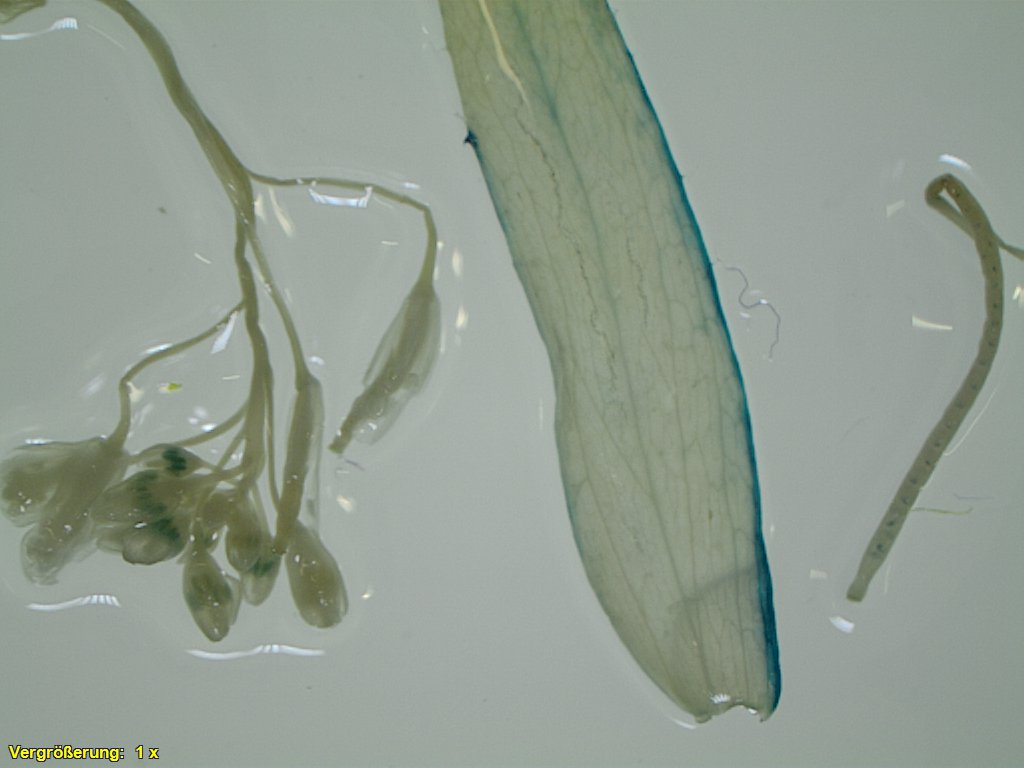
\includegraphics[width=\textwidth]{DR5_O+A.jpg}
				\caption{adulte Pflanze}
				\label{fig:DR5_Färbung}
			\end{subfigure}
			\hfill
			\begin{subfigure}[b]{0.45\textwidth}
				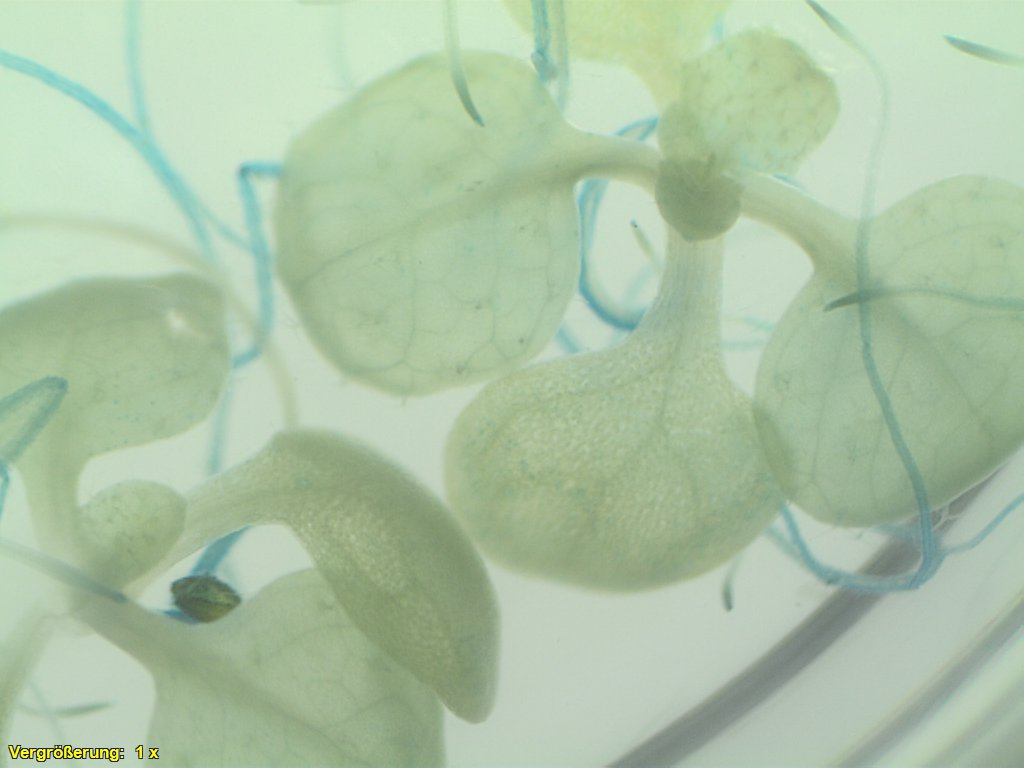
\includegraphics[width=\textwidth]{DR5_DP_O+A.jpg}
				\caption{Keimling-Dauerpräparat}
				\label{fig:DR5_DP}
			\end{subfigure}
			\caption{Mit GUS-Färbung angefärbte Infloreszenzen, Schote und Blatt von DR5-transgener Arabidopsis thaliana (\ref{fig:DR5_Färbung}) und vorgefärbte Keimlings Dauerpräparat (\ref{fig:DR5_DP})}
		\end{figure}

		\subsubsection{Cytokininaktivität}
		Mittels GUS-Färbung konnten die Gewebeteile, die eine Cytokininaktivität zeigen, angefärbt werden. Nach Betrachtung unter dem Stereo-Mikroskop ist zu erkennen, dass vor allem die Leitbündel der Blätter eine Färbung zeigten (Figure \ref{fig:cytokinin_TCS_Färbung}, Rechts). Die Infloreszenzen hingegen zeigt eine starke Färbung in den Blütenböden, die als kleine Punkte sichtbar waren. (siehe Figure \ref{fig:cytokinin_TCS_Färbung}, links). Bei der Frucht (Schote) konnte keine eindeutige Färbung ausgemacht werden. Es konnte jedoch eine leichte Zunahme der Färbung von der Narbe hin zum Fruchtstiel, beobachtet werden (siehe Figure \ref{fig:cytokinin_TCS_Färbung} Mitte).\\
		Anhand der zur Verfügung gestellten Dauerpräparate konnte man ebenfalls die Cytokininaktivität in anderen Pflanzenteilen erkennen. Hier waren vor allem die Wurzeln stark gefärbt, jedoch nicht die Wurzelspitze (siehe Figure \ref{fig:cytokinin_Dauerpräparat}). Zusätzlich zeigte sich, wie auch in der vorherigen Probe eine Färbung der Leitbündel der Blätter. 
		
		\begin{figure}[H]
			\centering
			\begin{subfigure}[b]{0.45\textwidth}
				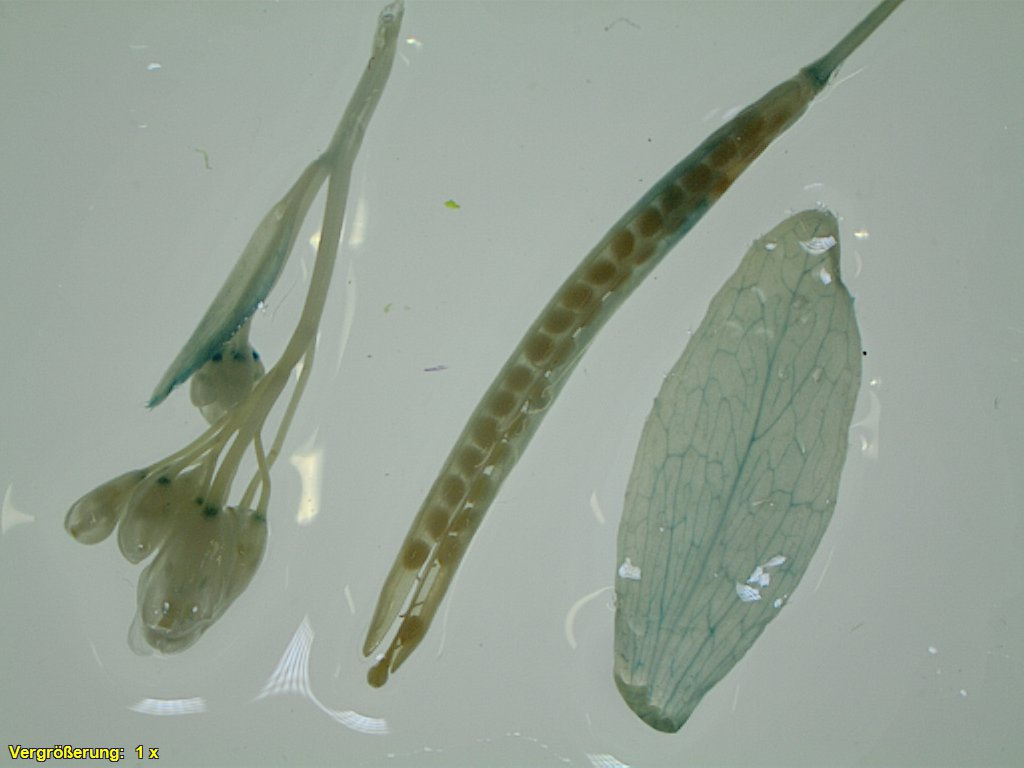
\includegraphics[width=\textwidth]{TCS_O+A.jpg}
				\caption{adulte Pflanze}
				\label{fig:cytokinin_TCS_Färbung}
			\end{subfigure}
			\hfill
			\begin{subfigure}[b]{0.45\textwidth}
				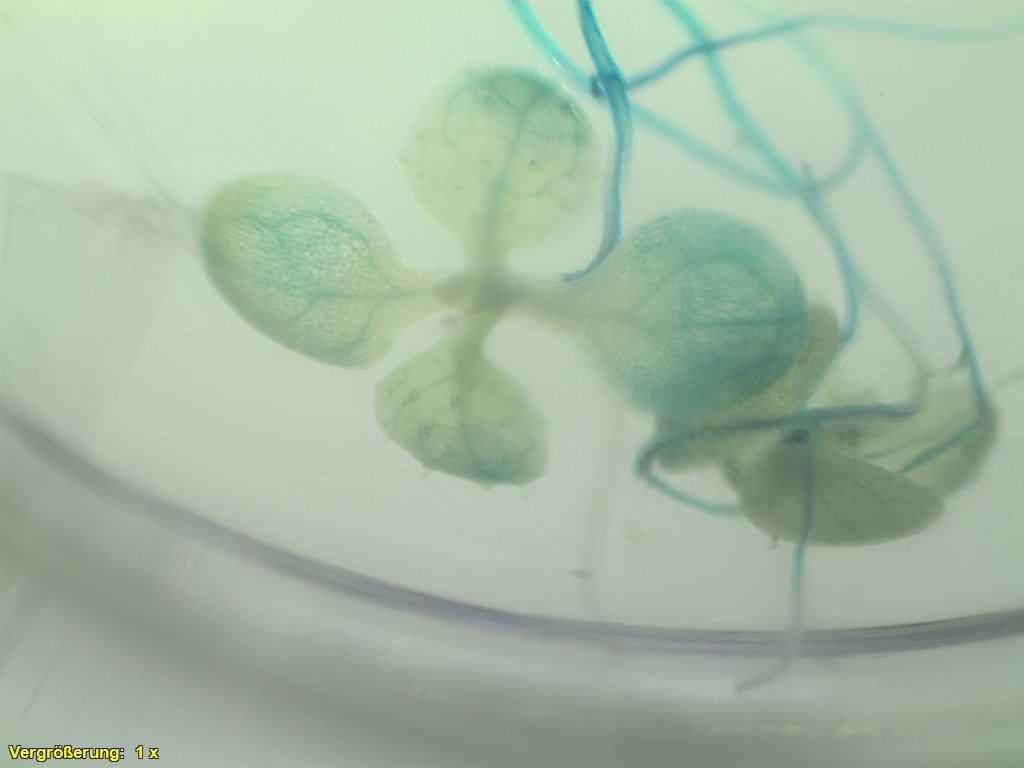
\includegraphics[width=\textwidth]{TCS_DP_O+A.jpg}
				\caption{Keimling-Dauerpräparat}
				\label{fig:cytokinin_Dauerpräparat}
			\end{subfigure}
			\caption{Mit GUS-Färbung angefärbte Infloreszenzen, Schote und Blatt von TCS-transgener Arabidopsis thaliana (\ref{fig:cytokinin_TCS_Färbung}) und vorgefärbte Keimlings Dauerpräparat (\ref{fig:cytokinin_Dauerpräparat})}
		\end{figure}
		
		
	\subsection{Phänotypische Analyse der Blüte}
	
		\begin{figure}[H]
			\centering
			\begin{subfigure}[b]{0.45\textwidth}
				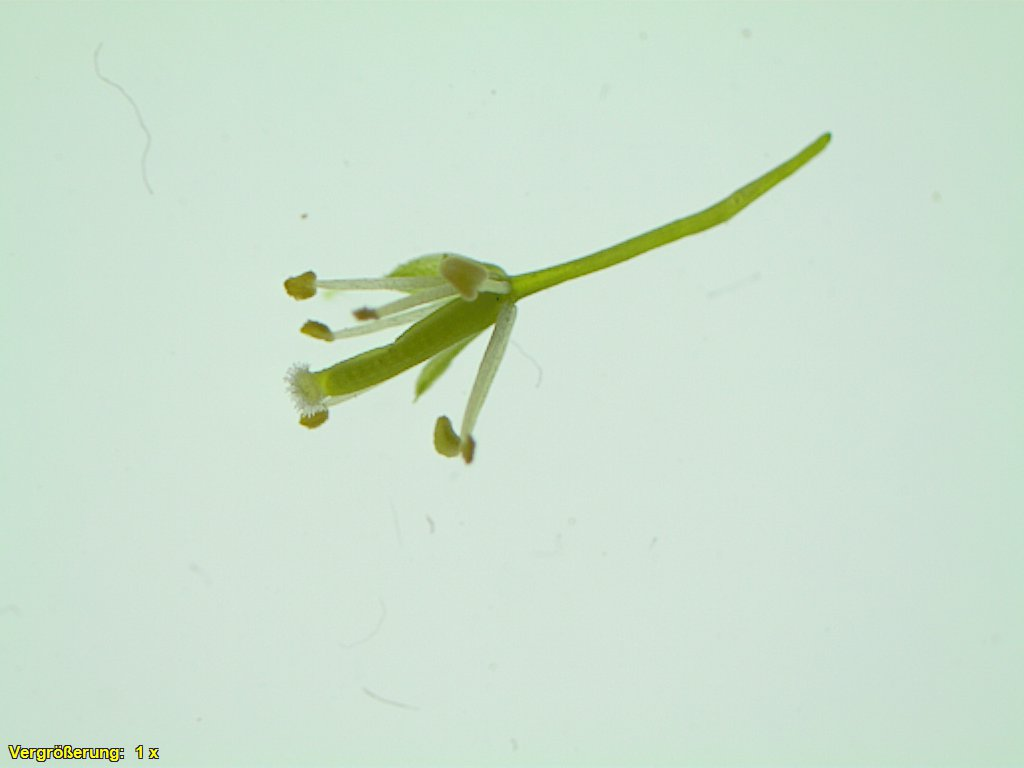
\includegraphics[width=\textwidth]{1_O+A.jpg}
				\caption{Mutant 1}
				\label{fig:M1}
			\end{subfigure}
			\hfill
			\begin{subfigure}[b]{0.45\textwidth}
				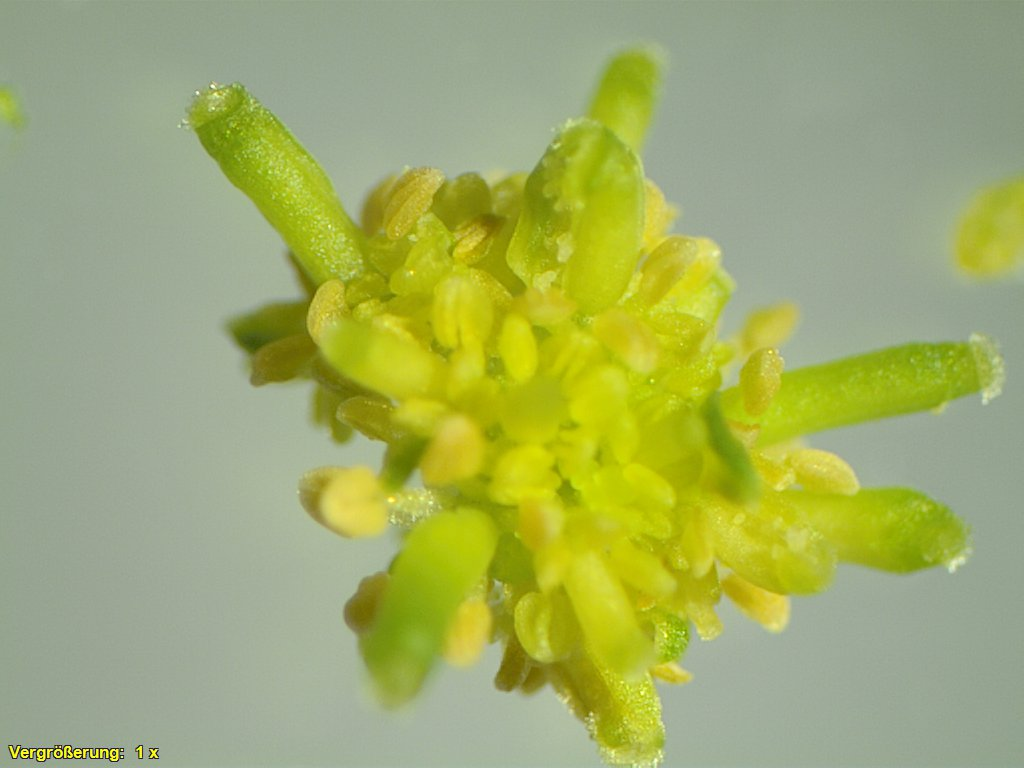
\includegraphics[width=\textwidth]{2_O+A(1).jpg}
				\caption{Mutant 2}
				\label{fig:M2}
			\end{subfigure}
			\hfill
			\begin{subfigure}[b]{0.45\textwidth}
				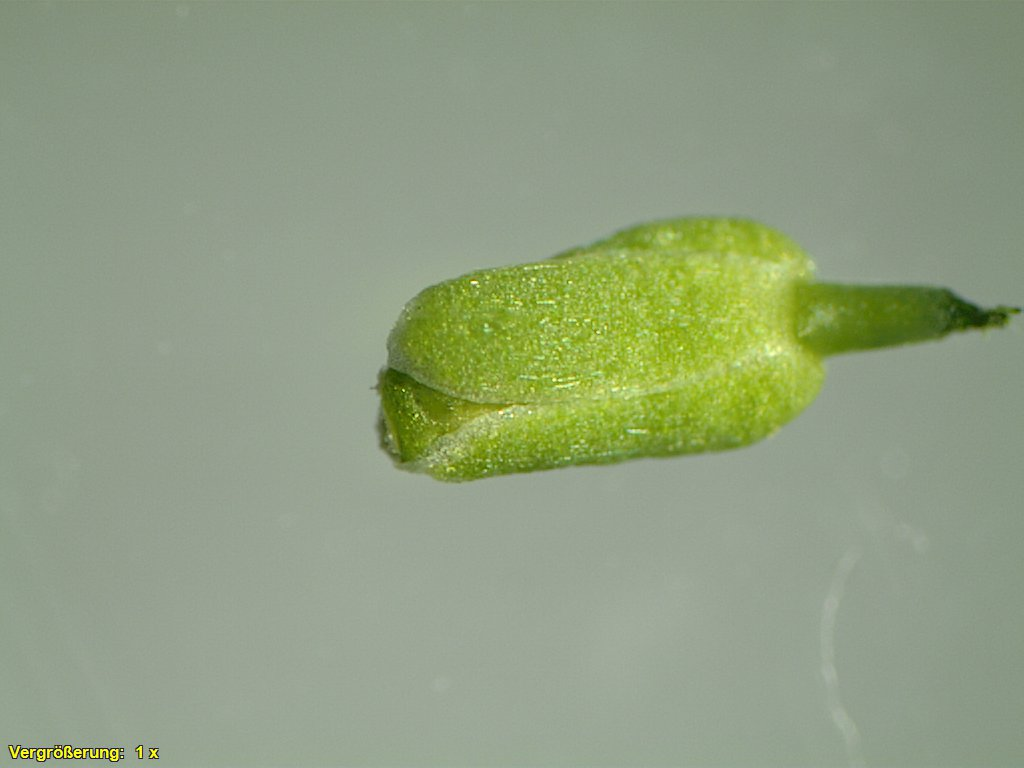
\includegraphics[width=\textwidth]{3_O+A(MU).jpg}
				\caption{Mutant 3}
				\label{fig:M3}
			\end{subfigure}
			\hfill
			\begin{subfigure}[b]{0.45\textwidth}
				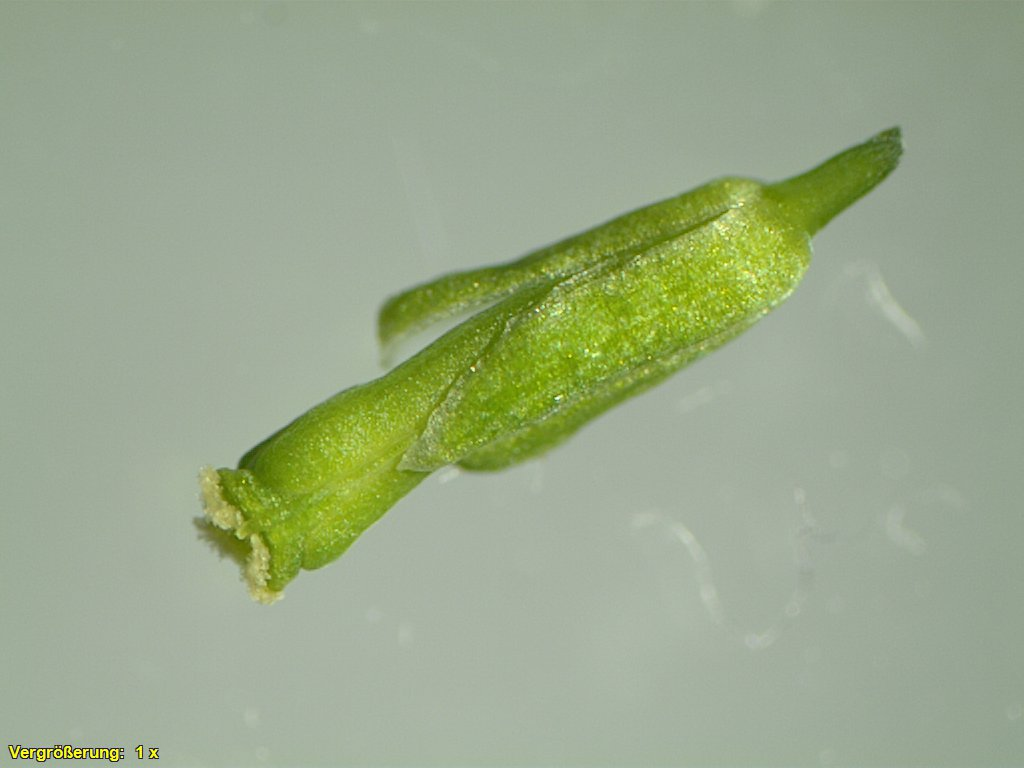
\includegraphics[width=\textwidth]{4_O+A(MU).jpg}
				\caption{Mutant 4}
				\label{fig:M4}
			\end{subfigure}
			\hfill
			\begin{subfigure}[b]{0.45\textwidth}
				\centering
				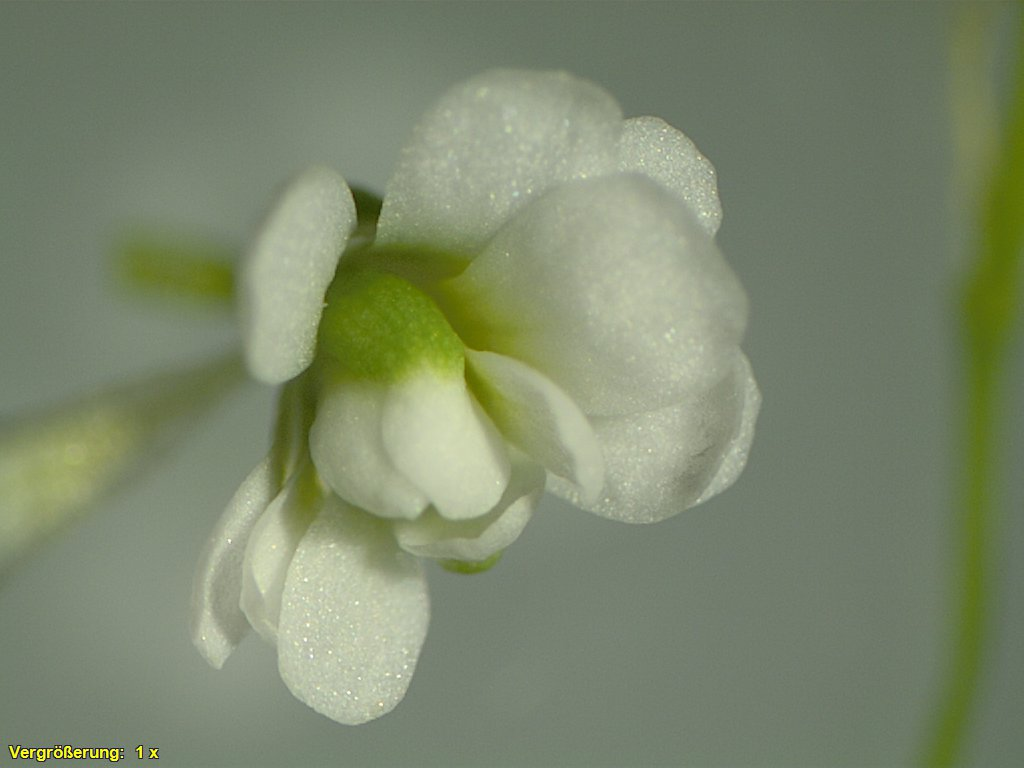
\includegraphics[width=\textwidth]{5_O+A(MU).jpg}
				\caption{Mutant 5}
				\label{fig:M5}
			\end{subfigure}
			\caption{Stereomikroskopische Aufnahme der Blüten von der Arabidopsis thalinana Mutanten 1-5 in der 1x-Vergrößerung}
			\label{Mutant}
		\end{figure}
		
		Die Mutante 1 besitzt Staub- und Fruchtblätter (siehe Figure \ref{fig:M1}).
		Die Mutante 2 besitzt ebenfalls nur Staub- und Fruchtblätter mit zusätzlich einer ausgeprägten Infloreszenzmeristem(siehe Figure \ref{fig:M2}).\\
		In Figure \ref{fig:M3} ist in der Mutant 3 zu sehen, dass die Fruchtblätter nur von Kelchblätter umgeben ist, welches phänotypisch auch Mutant 4 vorweist (siehe Figure \ref{M4}).\\
		Die Mutante 5 besitzt Kelchblätter, die in Figure \ref{fig:M5} nicht gut zu sehen ist und viele Kronblätter Kronenblätter.
		In Tab \refeq{tab:Mutatn ABC} ist dargestellt welche ABC-Gene aus den ABC-Klassen in den jeweiligen Mutanten 1-5 fehlen.
		
		\begin{table}[H]
			\centering
			\caption{ABC-Mutantenzuordnung von Arabidopsis thalinana - Mutante aus Figure \ref{Mutant}}
			\label{tab:Mutatn ABC}
			\begin{tabular}{cccccc}
				\toprule
				Mutant & 1 & 2 & 3 & 4 & 5\\
		 		Mutation & A$\ominus$ & A$\ominus$ & B$\ominus$ & B$\ominus$ & C$\ominus$ \\

				\bottomrule
			\end{tabular}
		\end{table}
		

	\section{Diskussion}
	
	\subsection{Auxin-und Cytokininaktivität}
	\subsubsection{Auxinaktivität}
	Auxin gehört zu den Phytohormen die bei den Pflanzen für den Wachstum, Tropismus, Verzweigung, Musterbildungsprozessen und Stammzellenidentität zuständig ist.\\
	Die hohe Konzentration von Auxin in den Staubblättern erklärt sich durch den erhöhten Bedarf an Pollenbildung während der sexuellen Phase des Lebenszykluses. Analog dazu fungiert die Anhäufung des Auxins in den Samen der Schoten. \\
	In den Blättern dient Auxin dem lateralen Wachstum, da dieses oft asymmetrisch verläuft, war hier eine sehr hohe Konzentration am rechten und eine verhältnissmäßig geringe am linken Rand zu beobachten. Die Keimlinge wiesen vor allem in Spross und Wurzeln hohe Auxinkonzentrationen auf, dies erklärt sich durch die Rolle von Auxin im Gravitropismus, der dafür sorgt, dass die Wurzeln nach unten, in den Boden, und der Spross nach oben wächst.\\
	Um die Auxin Aktivität noch deutlicher darstellen zu können, hätte es sich potenziell bewährt, die Proben länger zu färben und entfärben.
	\subsubsection{Cytokininaktivität}
	In den mit GAU-Färbelösung angefärbten Pflanzenteilen und im Fertigpräparat konnten Färbungen in verschiedenen Bereichen beobachtet werden. Eine eindeutige Färbung konnte im Leitgewebe des Blatts, im Blütenboden der Infloreszenzen, und in den Wurzeln erkannt werden. \\
	Nicht eindeutig war hingegen die Färbung der Schote. Eine Färbung trat überall dort auf, wo Cytokinin vorhanden war. Die Färbung der Wurzeln kann durch den Entstehungsort von Cytokinin erklärt werden. Vor allem in jungen Pflanzen wird Cytokinin hauptsächlich in den Wurzelspitzen gebildet und von dort über das Gefäßsystem in der Pflanze verteilt. Adulte Pflanzen bilden vor allem in meristematisch aktivem Gewebe, darunter Kambium, Vegetationspunkten und jungen Blättern, Cytokinin\cite{Schopfer}. Da es sich bei den Dauerpräparaten um Keimlinge handelte, lässt sich damit die hohe CK-Aktivität in den Wurzeln erklären. Cytokinin  ist an der Steuerung der Entwicklung und Lebensspanne von Blättern beteiligt. Schon in der Steuerung der Entwicklung vom shoot apical meristem (SAM) spielt Cytokinin eine wichtige Rolle. Im Sprossapikalmeristem (abgekürzt: SAM) wirkt es vor allem antagonistisch gegen die vom Auxin induzierte Blatt-Ausdifferenzierung und sorgt für eine gleichbleibende SAM-Aktivität. Dabei korreliert die Cytokininkonzentration mit der Größe des SEM. Auch in der Blattentwicklung hat Cytokinin einen Einfluss auf die Blattgröße durch Kontrolle der Zellteilung und des Zellwachstums. Der Alterungsprozess von Blättern wird auch durch die Cytokininkonzentration mitbestimmt. \\
	So kommt es bei einer sinkenden Cytokininkonzentration zu einem schnelleren Alterungsprozess der Blätter\cite{Wu_Wenqi;}. All diese Erkenntnisse können als Grund für die deutlich sichtbare GAU-Färbung der Blatt-Leitgewebe angeführt werden. Sowohl für die jungen Blätter, die sich noch in der Entwicklung befinden, als auch für die adulten Blätter, bei denen Cytokinin die Seneszenz verzögert, spielt Cytokinin eine wichtige Rolle. Interessant wäre auch eine Untersuchung der Cytokininkonzentration in Blättern, bei denen bereits Seneszenz Prozesse eingesetzt haben. In der Blütenentwicklung hat Cytokinin nicht nur einen positiven Einfluss auf die Größe der gebildeten Blütenorgane, sondern auch auf die Anzahl von gebildeten Samenanlangen \cite{Cytokininregulation}. \\
	Die punktförmige Cytokininkonzentration im Blütenboden lässt sich dadurch erklären, dass sich hier das Blütenmeristem befindet. Wie bereits oben erwähnt wird in den meristematisch aktiven Geweben Cytokinin produziert, weshalb hier eine besonders hohe Konzentration zu finden ist.
	
	\subsection{Floral homöotische Gene}
	Für die Blütenorganbildung sind sogenannte floral homöotische Gene verantwortlich, dessen Funktion in drei Klassen eingeteilt werden kann. Die drei Klassen wurden in einem ABC-Modell beschrieben, das beschreibt welchen Einfluss sie jeweils in der Blütenbildung haben (Figure \ref{fig:floralgene_Wildtyp}).\\ 
	Würde eine Gen-Klasse in der Arabidopsis Pflanze fehlen, dann können gewisse Blütenblätterorgane nicht mehr gebildet werden (Figure \ref{blütendiagramm mutation}).
	Bei der Mutation 1 (siehe Figure \ref{fig:M1}) handelt es sich um eine A$\ominus$-Mutant, da diese nur aus Frucht- und Staubblätter besteht. Die C-Klassegene werden nicht durch die A-Klassegene inhibiert und kann somit die Kelch- und Kronenblätterbildung selbst inhibieren.\\
	Interessanterweise besitzt die Mutante 1 nicht viel mehr Staub- und Fruchtblätter als der Wildtyp.\\
	Mutante 2 (siehe Figure \ref{fig:M2}) ist ebenfalls eine A$\ominus$-Mutant, mit einer sehr ausgeprägten Influoreszenzmeristem. Hier musst die Pflanze selber noch eine andere Genmutation besitzen, die sich phänotypisch ausprägt.\\
	Die Mutante 3 und 4 sind beide B$\ominus$-Mutante, die nicht übermäßig mehr Kelch- und Fruchtblätter aufweisen wie der Wildtyp (siehe Figure \ref{fig:M3} und \ref{fig:M4}).
	Hingegen Mutant 5 besitzt mehr als 4 Kronenblätter als der Wildtyp(siehe Figure \ref{fig:M5}). Leider wurde in diesen Versuch die Kelchblätter nicht gezählt, so dass die Zahl grob mit mehr als 4 Kelchblätter vom Foto beurteilt werden muss.\\
	Anhand des Phänotyps kann nicht genau beurteilt werden, welche Genklasse für die Repression von Cytokinin verantwortlich ist oder welchen Einfluss Auxin in der Blütenbildung hat.
	Eine Vollständige Genanalyse würde diese Fragestellung eventuell beantworten können.
	
	
		\begin{figure}[H]
			\centering
			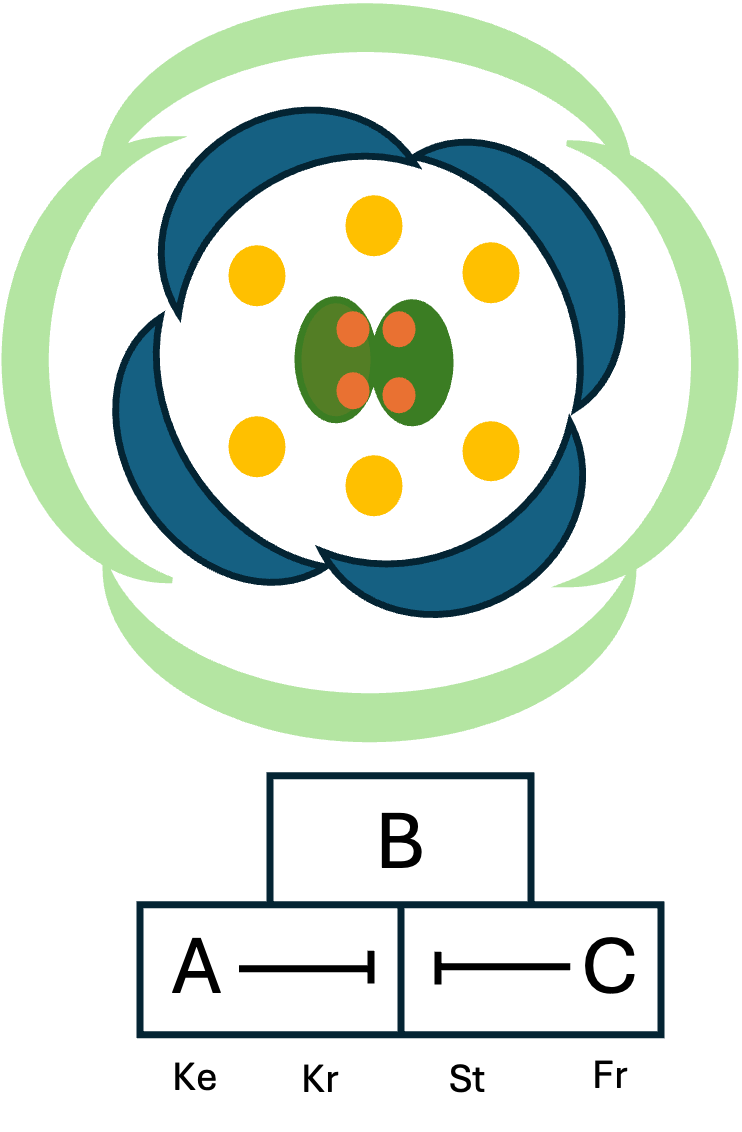
\includegraphics[scale=0.85]{Wildtyp_diagramm.png}
			\caption{ABC-Modell desFloral homöotische Gen als Diagramm des Wildtypes und Blütendiagramm vom Brassicaceae.\\
			Kr = Krone, Ke = Kelch, St = Staub, Fr = Frucht -Blätter}
			\label{fig:floralgene_Wildtyp}
		\end{figure}
	
		\begin{figure}[H]
			\centering
			\begin{subfigure}[b]{0.25\textwidth}
				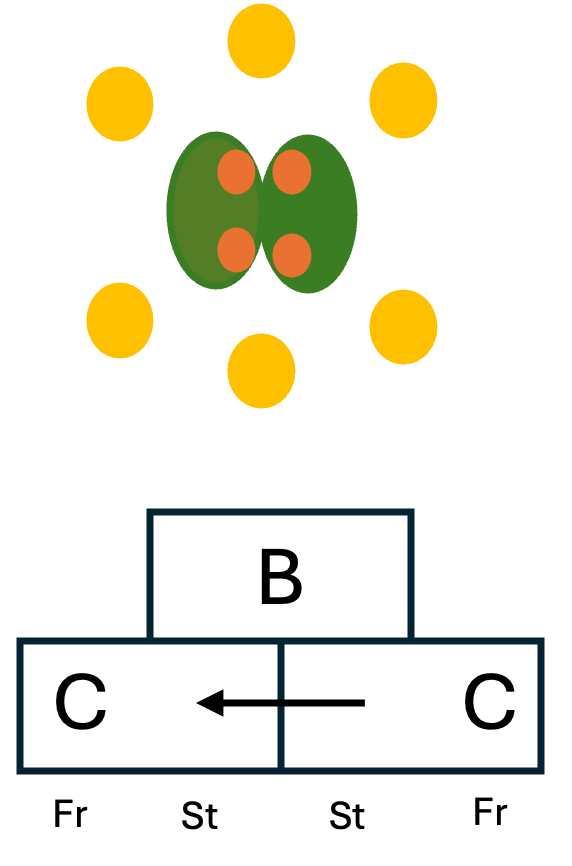
\includegraphics[width=\textwidth]{A-Typ_diagramm.png}
				\caption{A$\ominus$-Mutant}
				\label{fig:A-Mutant}
			\end{subfigure}
			\hfill
			\begin{subfigure}[b]{0.3\textwidth}
				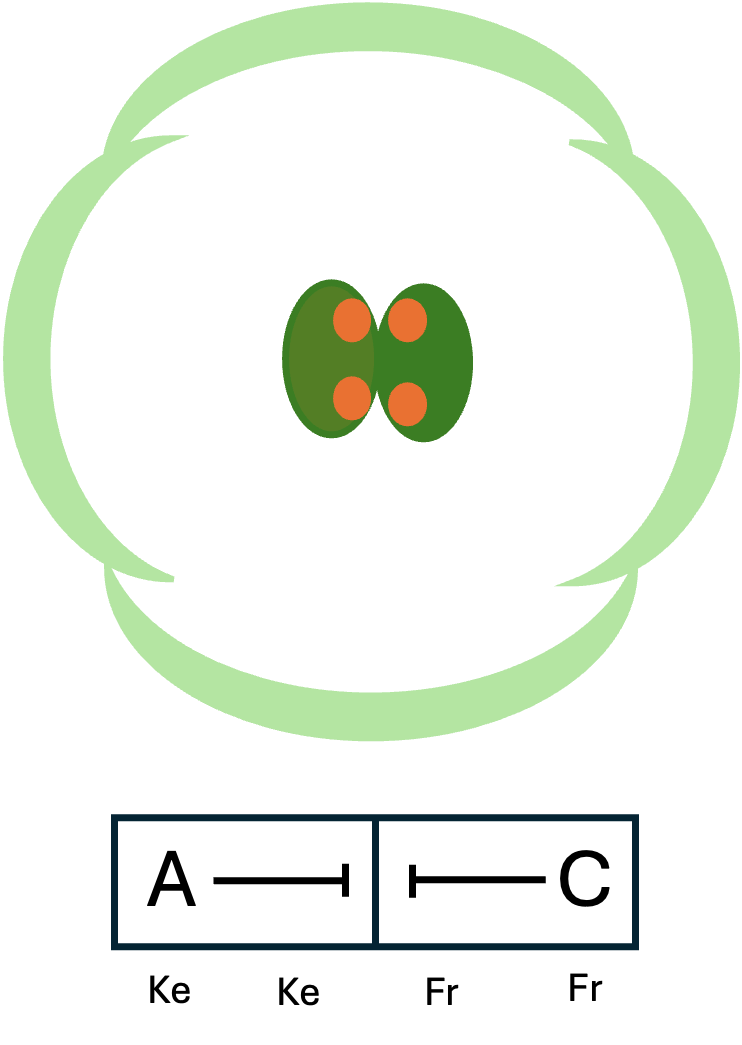
\includegraphics[width=\textwidth]{B-Mutant_diagramm.png}
				\caption{B$\ominus$-Mutant}
				\label{fig:B-Mutant}
			\end{subfigure}
			\hfill
			\begin{subfigure}[b]{0.3\textwidth}
				\includegraphics[width=\textwidth]{C-Mutant_diagramm.png}
				\caption{C$\ominus$-Mutant}
				\label{fig:C-Mutant}
			\end{subfigure}
	
			\caption{ABC-Modell angewant auf verschiedene Mutationstypen und deren Blütendiagramm}
			\label{blütendiagramm mutation}
		\end{figure}
		
		

	\section{Anhang}

	\addcontentsline{toc}{section}{References}
	\bibliographystyle{plainurl}
	\nocite{*}
	\bibliography{Literatur}
	\newpage

	
\end{document}